%----------------------------------------------------------------------------------------
%----------------------------------------------------------------------------------------
%----------------------------------------------------------------------------------------
%DATA
%----------------------------------------------------------------------------------------
%----------------------------------------------------------------------------------------
%----------------------------------------------------------------------------------------

\section{Sample of study}
\label{Sec: data_SOMN}

We gathered data from 10 regions in M31 (Fig.~\ref{fig: regions in m31}) and 8 regions in M101 (Fig.~\ref{fig: regions in m101}) as inputs for SOMs.
We chose those specific regions due to availability of the PAH observations for them.
Besides PAH data, for each galaxy, we chose spectroscopy and photometry observations as well as their derived properties, such as SFR, stellar mass, dust luminosity (L$_{\rm dust}$) and mass, metallicity, and gas mass.
Table~\ref{tab: data} shows the full list of the data and their unit for both M31 and M101.
We divided each value by the area of their region (in arcsec$^2$), to remove the distance factor from the data compare values of quantities in both galaxies.
Since the resolution of the data varies from less than 1$\arcsec$ to $60\arcsec \times 90 \arcsec$, any attempt to match the resolutions causes loosing all the information in some of the input data (e.g. the spectroscopic data).
On the other hand, in this project we used flux (or value of the quantities) per area as inputs of SOMs, which the convolution methods conserve~\citep{Aniano12}.
Therefore, we did not perform any resolution matching in this paper and used data in their original resolution.


\import{../sections/tables/}{tab_data.tex}

% \begin{figure}
%   \begin{subfigure}[b]{0.5\textwidth}
%         \centering
%     %\centering
%         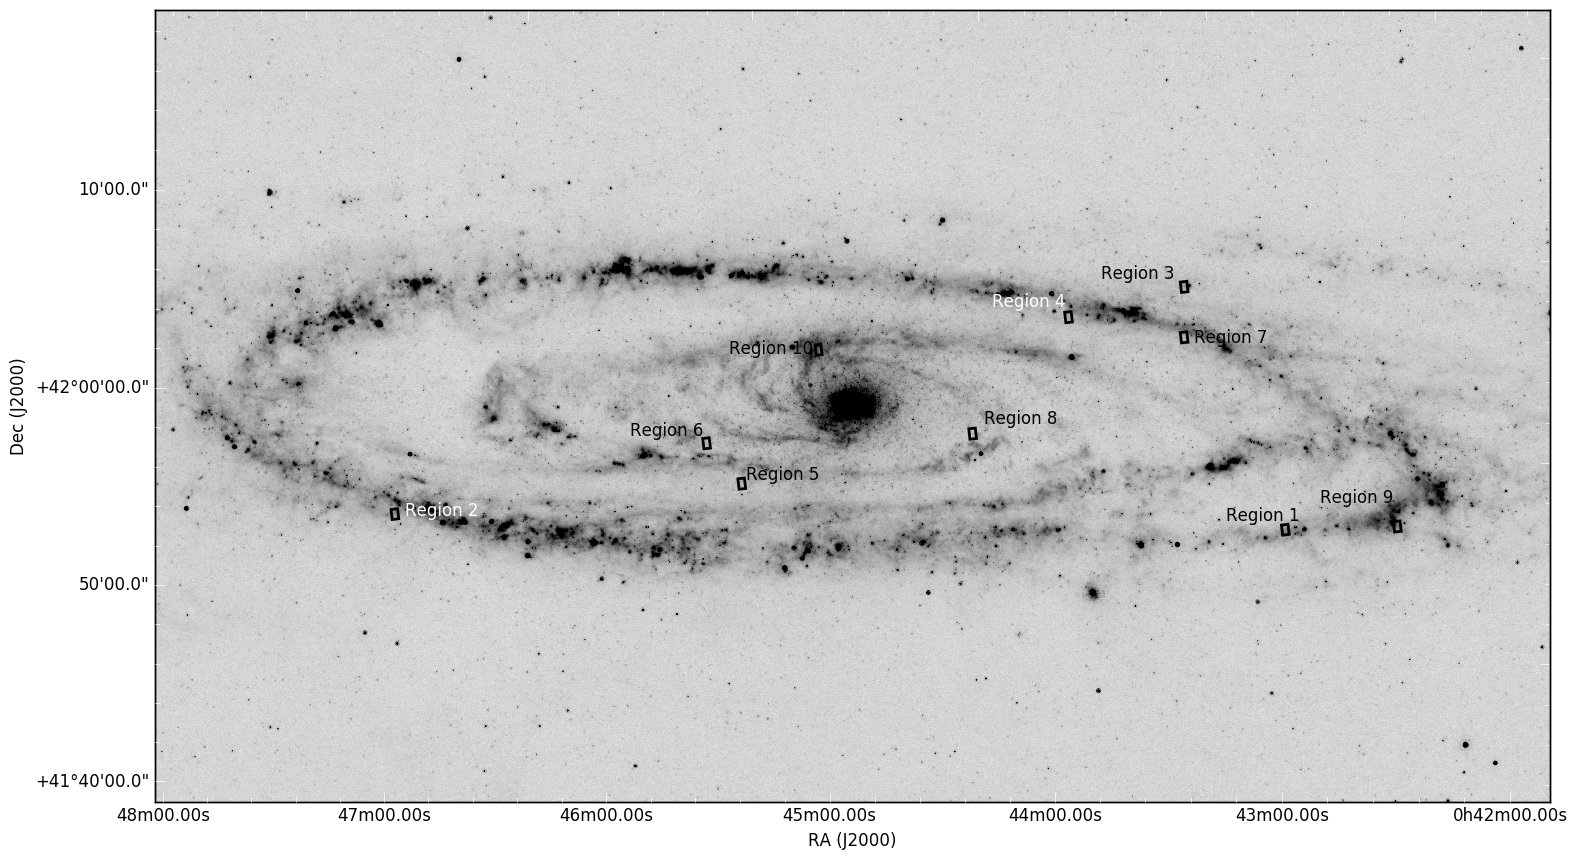
\includegraphics[width=0.97\textwidth]{../images0.0/M31/M31.png}
%         \caption{MIPS24 image of M31, with position of 10 regions that we studies.}
%         \label{fig: regions in m31}
%     \end{subfigure}
%     \hfill
%     \begin{subfigure}[b]{0.5\textwidth}
%         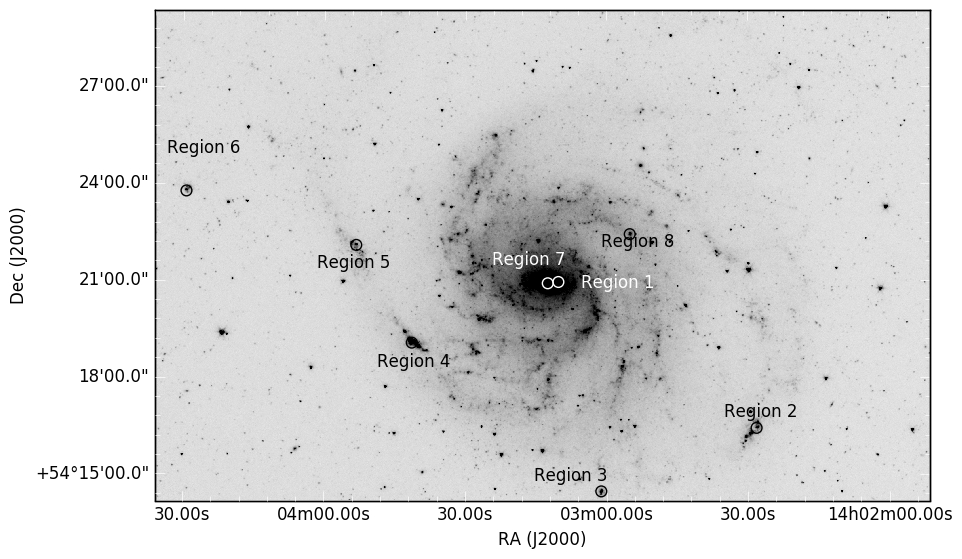
\includegraphics[width=\textwidth]{../images0.01/M101/M101.png}
%         \caption{IRAC1 image of M101, with position of our 8 regions that we studies.}
%     \label{fig: regions in m101}
%     \end{subfigure}
%     \caption{Position of the data in M31 (up) and M101 (down).}
% \end{figure}

  \begin{figure}
    \subfloat[MIPS 24~$\mu$m image of M31 from~\cite{Gordon06}, with position of 10 regions \label{fig: regions in m31}]{
      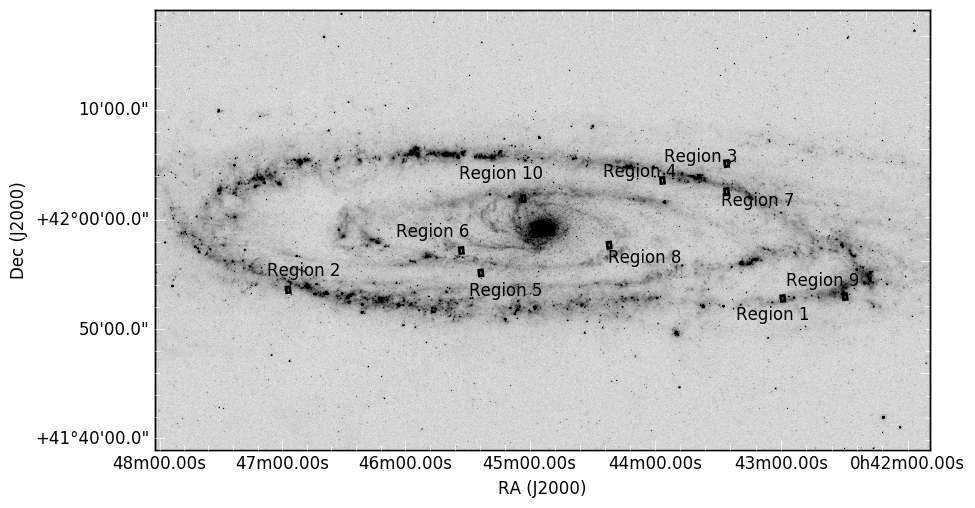
\includegraphics[width=0.5\textwidth]{../images0.01/M31/M31.png}
    }
    \hfill
    \subfloat[IRAC 3.6~$\mu$m image of M101~\citep{Dale09}, with position of 8 regions.\label{fig: regions in m101}]{
      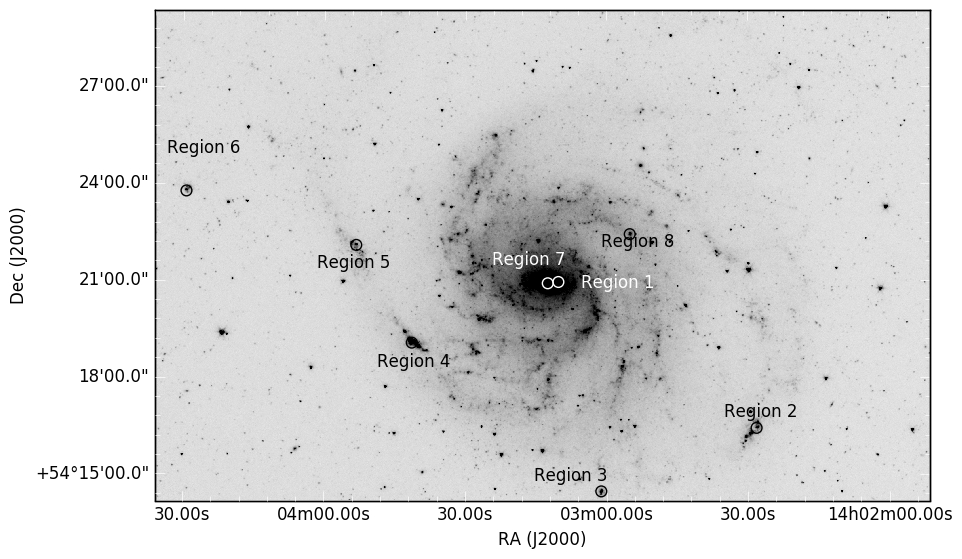
\includegraphics[width=0.5\textwidth]{../images0.01/M101/M101.png}}
    \caption{Position of regions that the input data for SOM that obtained from there in M31 (up) and M101 (down).}
    \label{fig:dummy}
  \end{figure}

%M31 data 
%%%%% Sahar: More detail, right?
    \subsection{M31 data}
     \label{Sec: data_M31_SOMN} 
     
     The 10 regions in M31 were chosen due to availability of the PAH data for them. 
     \cite{Dim15} studied PAH for those regions using {\it Spitzer}/IRS observations. 
     They used~{\sc PAHFIT IDL} tool~\citep{Smith07b} and measured fluxes and equivalent widths of PAH features as well as atomic line features.
     %For spectroscopy part of our sample, we utilized their measured fluxes for PAH lines. 
     \cite{Dim15} also measured metallicity and radiation hardness index (RHI) for these 10 regions.
     We used the measured fluxes for PAH featured, metallicity and RHI of each region as an input for SOMs.
     
 We used \GALEX FUV and NUV channels~\citep{Martin05}, \halpha, \sii~and \oiii narrow band~\citep{Massey07}, IRAC channels 1 to 4~\citep{Barmby06}, MIPS24 and 70~$\mu$m~\citep{Gordon06}, PACS100 and 160~$\mu$m and SPIRE250, 350, and 500~$\mu$m~\citep{Fritz12} emission for photometry part of the sample.
     We changed units of all fluxes to Wm$^{-2}$ to be the same unit as PAH fluxes.
     $^{12}$CO (J:$1\rightarrow0$) line~\citep{Nieten06} and the atomic gas (H\,{\sc I}) 21~cm emission from~\cite{Chemin09} were added to the input data. 
     For derived values, we utilized SFR(FUV + 24$\mu$m), stellar mass, mass of molecular clouds, mass of atomic gas (H\,{\sc I}), total gas mass, and total infrared (TIR) luminosity (L$_{\rm TIR}$) data from \cite{Rahmani16}, and L$_{\rm dust}$ and mass data from \cite{Draine14}.
     
    \subsection{M101 data}
    \label{Sec: data_M101_SOMN} 
     For M101, we used PAH fluxes which had been measured using {\sc PAHFIT IDL} tool and reported in \cite{Gordon08}.
     We also added their measurement of metallicity and RHI for these regions to our sample.
     We used data available on NED~\footnote{The NASA/IPAC Extragalactic Database (NED) is operated by the Jet Propulsion Laboratory, California Institute of Technology, under contract with the National Aeronautics and Space Administration.} website to gather our photometry data of M101. 
     We chose data from \GALEX FUV and NUV channels~\citep{depaz07}, IRAC channels 1 to 4, MIPS~24 and 70~$\mu$m~\cite{Dale09}, and  PACS~100 and 160~$\mu$m and SPIRE~250, 350, and 500~$\mu$m emission from~\cite{Kennicutt11}.
     Similar to M31 data, we used $^{12}$CO (J:$1\rightarrow0$) line~\citep{Helfer03} and the atomic gas (H\,{\sc I}) 21~cm emission from \cite{Walter08}.
     SFR(FUV + 24$\mu$m), stellar and total gas mass map were calculated using the same methods that M31 data were derived in~\cite{Rahmani16}.
     
     Some of the correlations between some wavelengths and properties of galaxies are well-known.
     Emission in 3.6$\mu$m band traces the old stellar population very well~\citep[e.g]{Leitherer99,Smith07a} and it is used to calculate the stellar mass~\citep{Eskew12}.
     FUV, \halpha, and TIR emission are some of indicators of star forming regions.
     In this project we used SFR traced by FUV emission which corrected for foreground stars using NUV emission and for dust extinction using 24$\mu$m emission.
     TIR emission is calculated from modified version of~\cite{Draine07} calibration using using 8, 24, 70, and 160 $\mu$m emission~\citep{Boquien10}.
     To make sure that we do not use the observed data as an input data in various forms, we removed all the observed data, that were used to calculate properties of the galaxies from the input sample.
     We used these sample as the main input for creating SOMs.
     Fig.~\ref{fig: cor_all} shows Pearson correlation coefficients with a confidence level of $95\%$ for the input data. 
     
     
      \begin{figure}
                \centering
                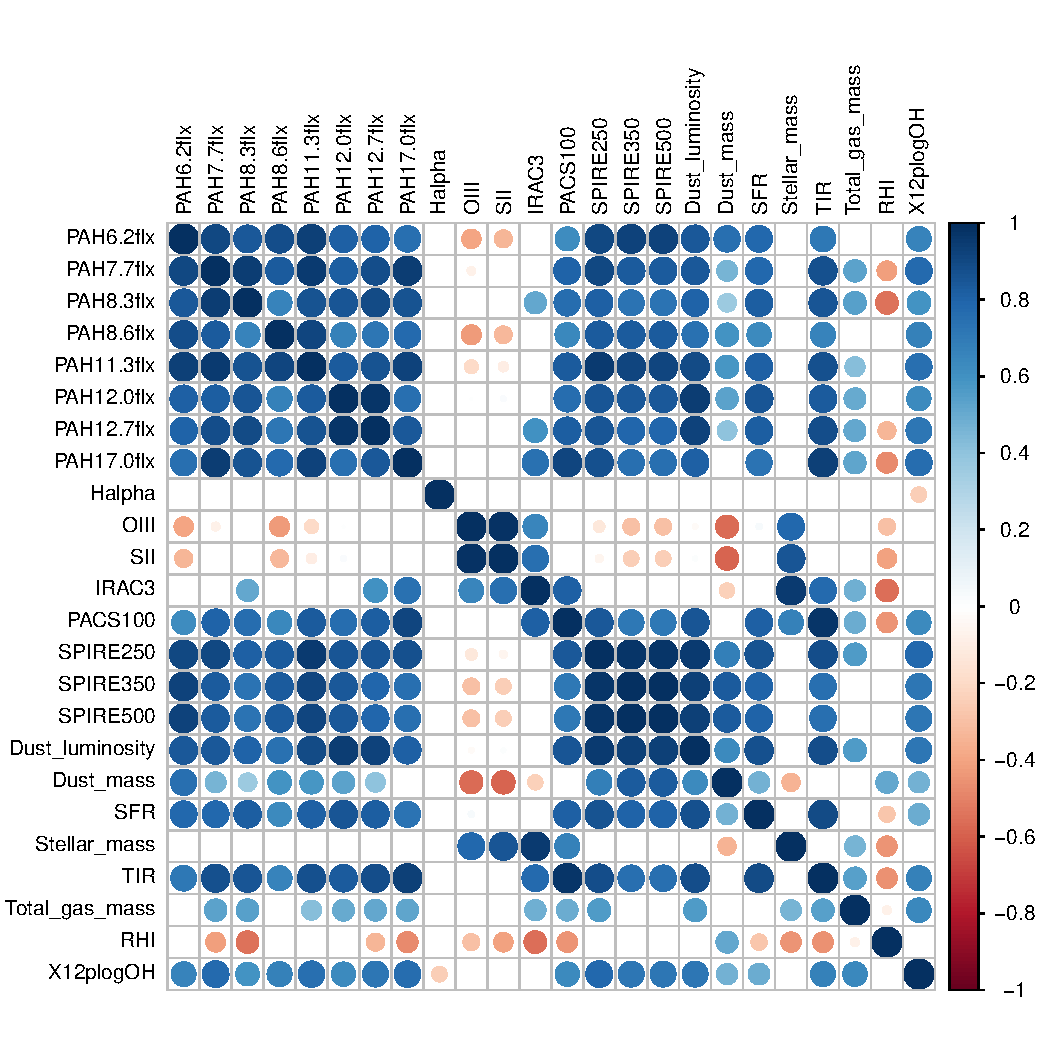
\includegraphics[width=0.5\textwidth]{../images0.01/cor_plots/M31_all_derived_ones_core_plot_for_paper.pdf}
            \caption{Pearson correlation coefficients with a confidence level of 95$\%$ for all the in the subset 0. The colours show the Pearson correlation coefficients where 1 means highly correlated and -1 is highly anti-correlated quantities. The non-significant correlations were left empty.}
            \label{fig: cor_all}
        \end{figure}
 
  